%*----------- SLIDE -------------------------------------------------------------
\begin{frame}[t]{O projeto} 

    O projeto \textbf{Warthog + AUM} consiste na integração de um robô manipulador UR5 com o robô UGV Warthog.

    \vspace*{0.3cm}
    %\newline
        \begin{columns}[t]
            \column{.05\linewidth}
            \column{.4\linewidth}
            \begin{center}
                O sistema deve permitir a manipulação do \textbf{AUM} enquanto o \textbf{Warthog} navega de forma autônoma.
            \end{center}
            \column{.6\linewidth}
            \begin{center}
            %\centerline{
                \begin{figure}
                    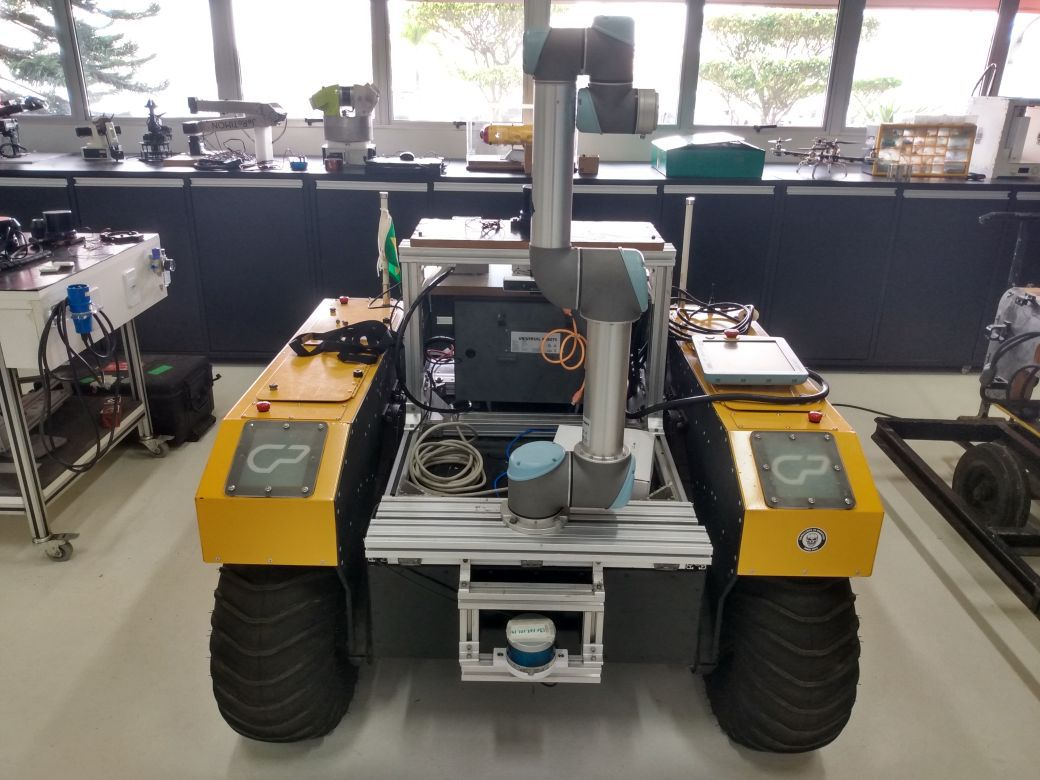
\includegraphics[width=.65\textwidth]{warthog+aum/full-system.jpg}
                    %\caption{Pista de corrida \cite{agostini2007}}
                \end{figure}
            %}
            \end{center}
        \end{columns}
%*----------- notes
    \note[item]{Notes can help you to remember important information. Turn on the notes option.}
\end{frame}
%-

%*----------- SLIDE -------------------------------------------------------------
\begin{frame}[t]{Justificativa} 

    \text  Existem muitas aplicações da robótica em áreas onde o uso de humanos é impraticável ou indesejável. Entre eles estão submarinos, exploração planetária, recuperação e reparo de satélites, as quais são situações que envolvem pertubações no meio.

    %\newline
        \begin{columns}[t]
            \column{.02\linewidth}

            \column{.3\linewidth}
            \begin{center}
                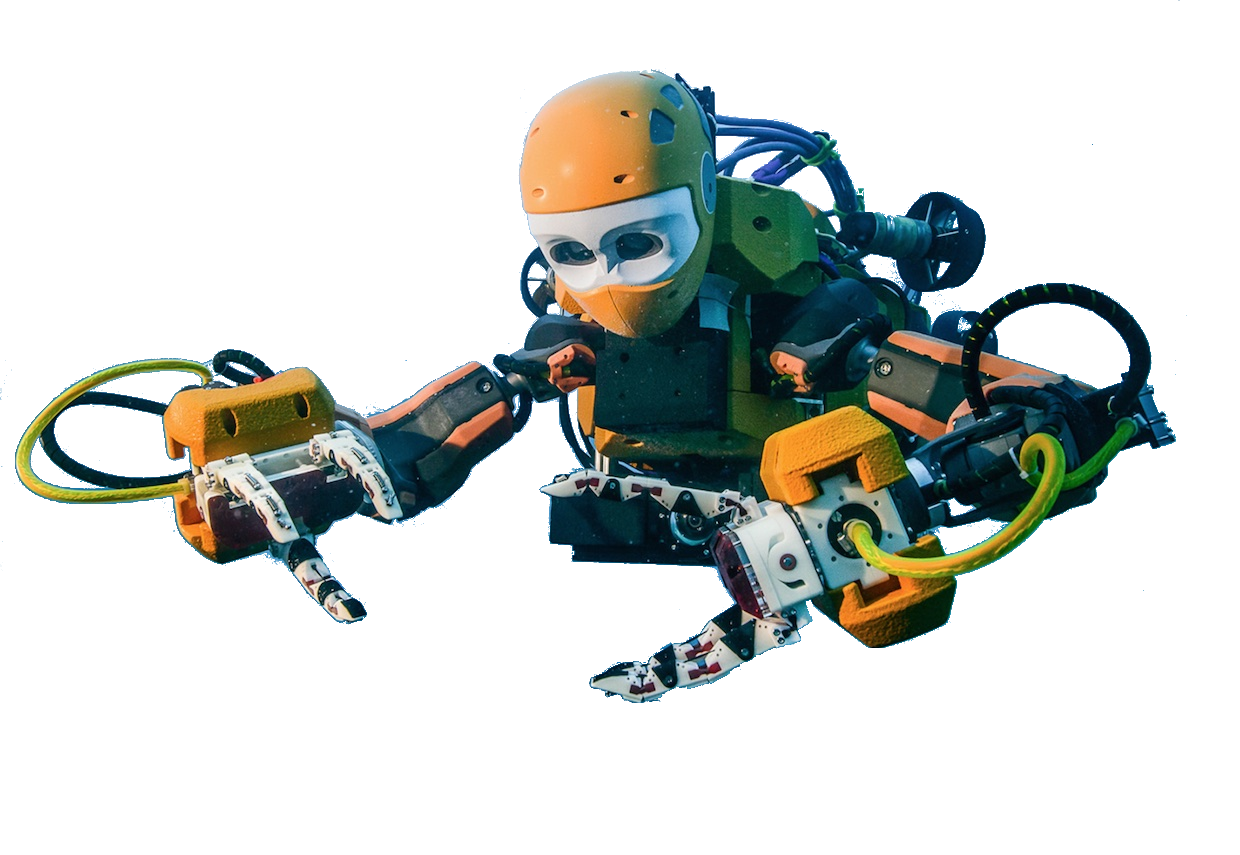
\includegraphics[width=.8\textwidth]{warthog+aum/robot.png}
            \end{center}

            \column{.3\linewidth}
            \begin{center}
                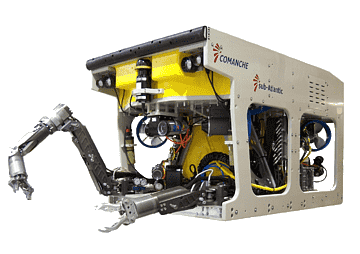
\includegraphics[width=.65\textwidth]{warthog+aum/rov-aum.png}
            \end{center}

            \column{.3\linewidth}
            \begin{center}
                \begin{figure}
                    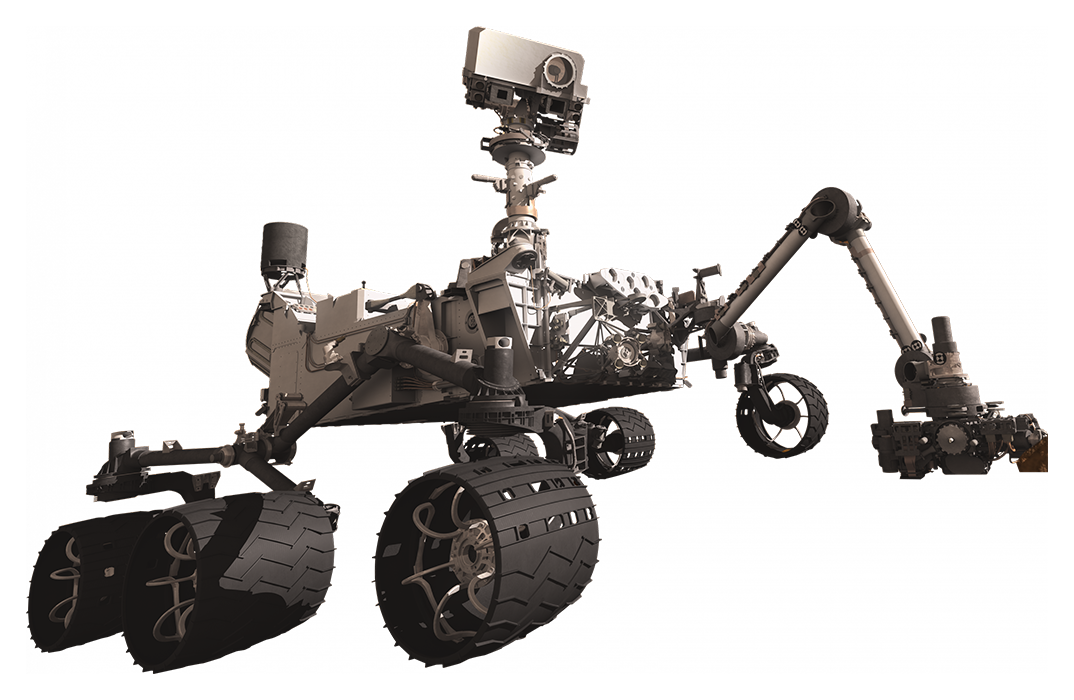
\includegraphics[width=.65\textwidth]{warthog+aum/curiosity.png}
                \end{figure}
            \end{center}

        \end{columns}
        O projeto \textbf{Warthog + AUM} visa o desenvolvimento de um modelo para a compensação das pertubações sofridas por manipuladores utilizados acoplados em robôs móveis.
%*----------- notes
    \note[item]{Notes can help you to remember important information. Turn on the notes option.}
\end{frame}
%-

%*----------- SLIDE -------------------------------------------------------------
\begin{frame}[t]{Etapas de desenvolvimento do projeto} 
   
    \begin{columns}[t]
        \column{.01\linewidth}

        \column{.2\linewidth}
        \begin{center}
            Modelo do robô na simulação
            \begin{figure}
            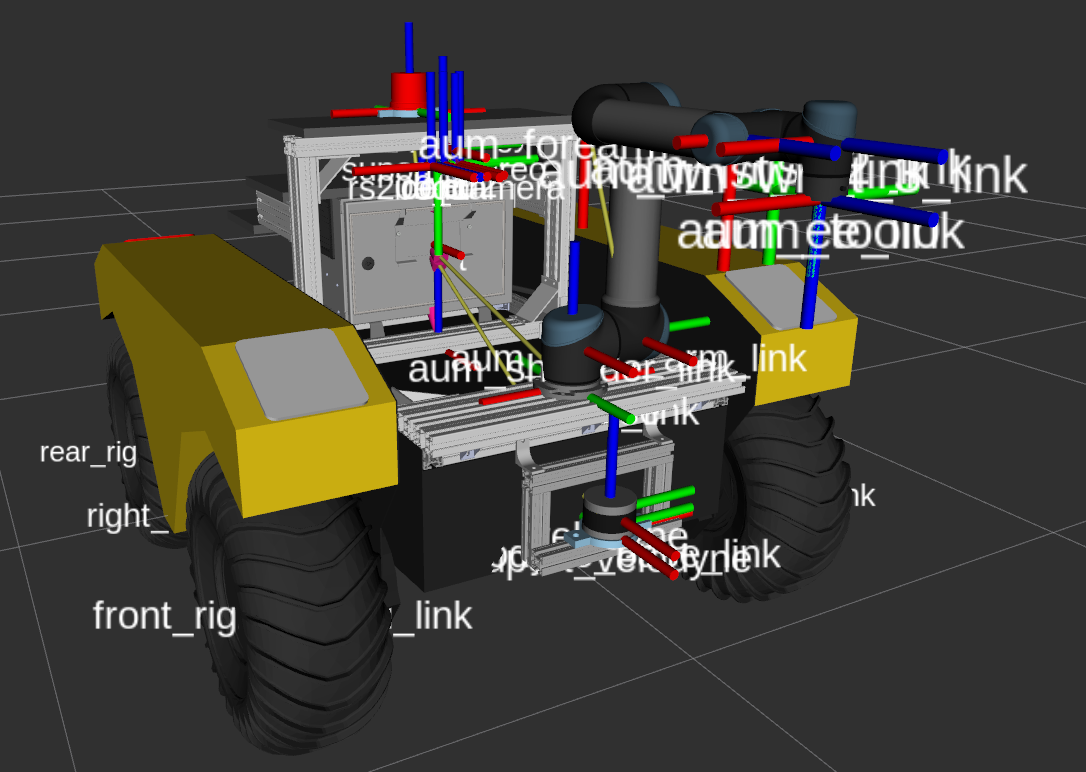
\includegraphics[width=.9\textwidth]{warthog+aum/Captura_de_tela_de_2021-09-29_09-22-23.png}
        \end{figure}
        \end{center}

        \column{.2\linewidth}
        \begin{center}
            Montagem do sistema
            \begin{figure}
            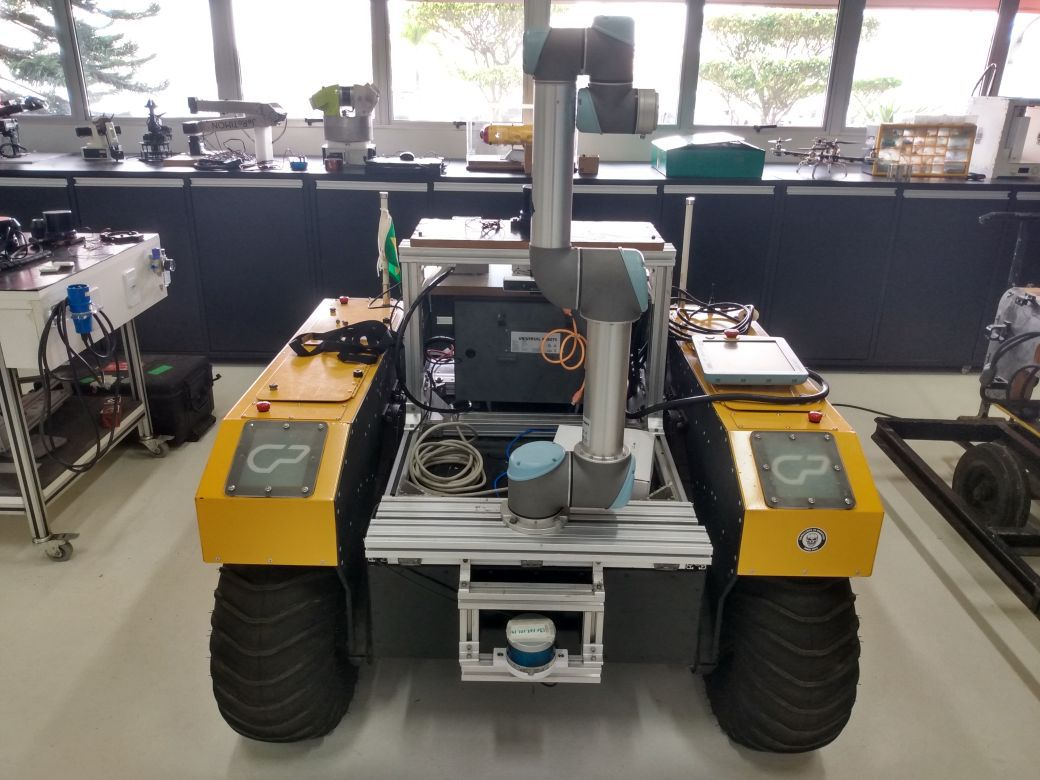
\includegraphics[width=.9\textwidth]{warthog+aum/full-system.jpg}
        \end{figure}
        \end{center}

        \column{.2\linewidth}
        \begin{center}
            Painel de testes na simulação
            \begin{figure}
                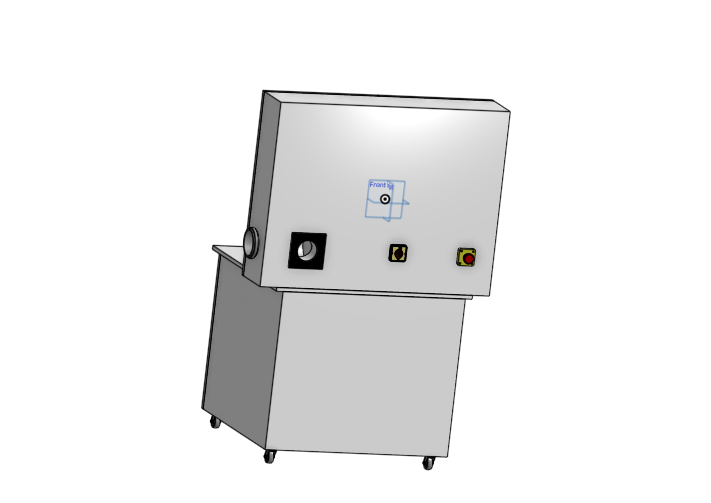
\includegraphics[width=.9\textwidth]{warthog+aum/aruco.png}
            \end{figure}
        \end{center}

        \column{.2\linewidth}
        \begin{center}
            Montagem do painel de testes
            \begin{figure}
                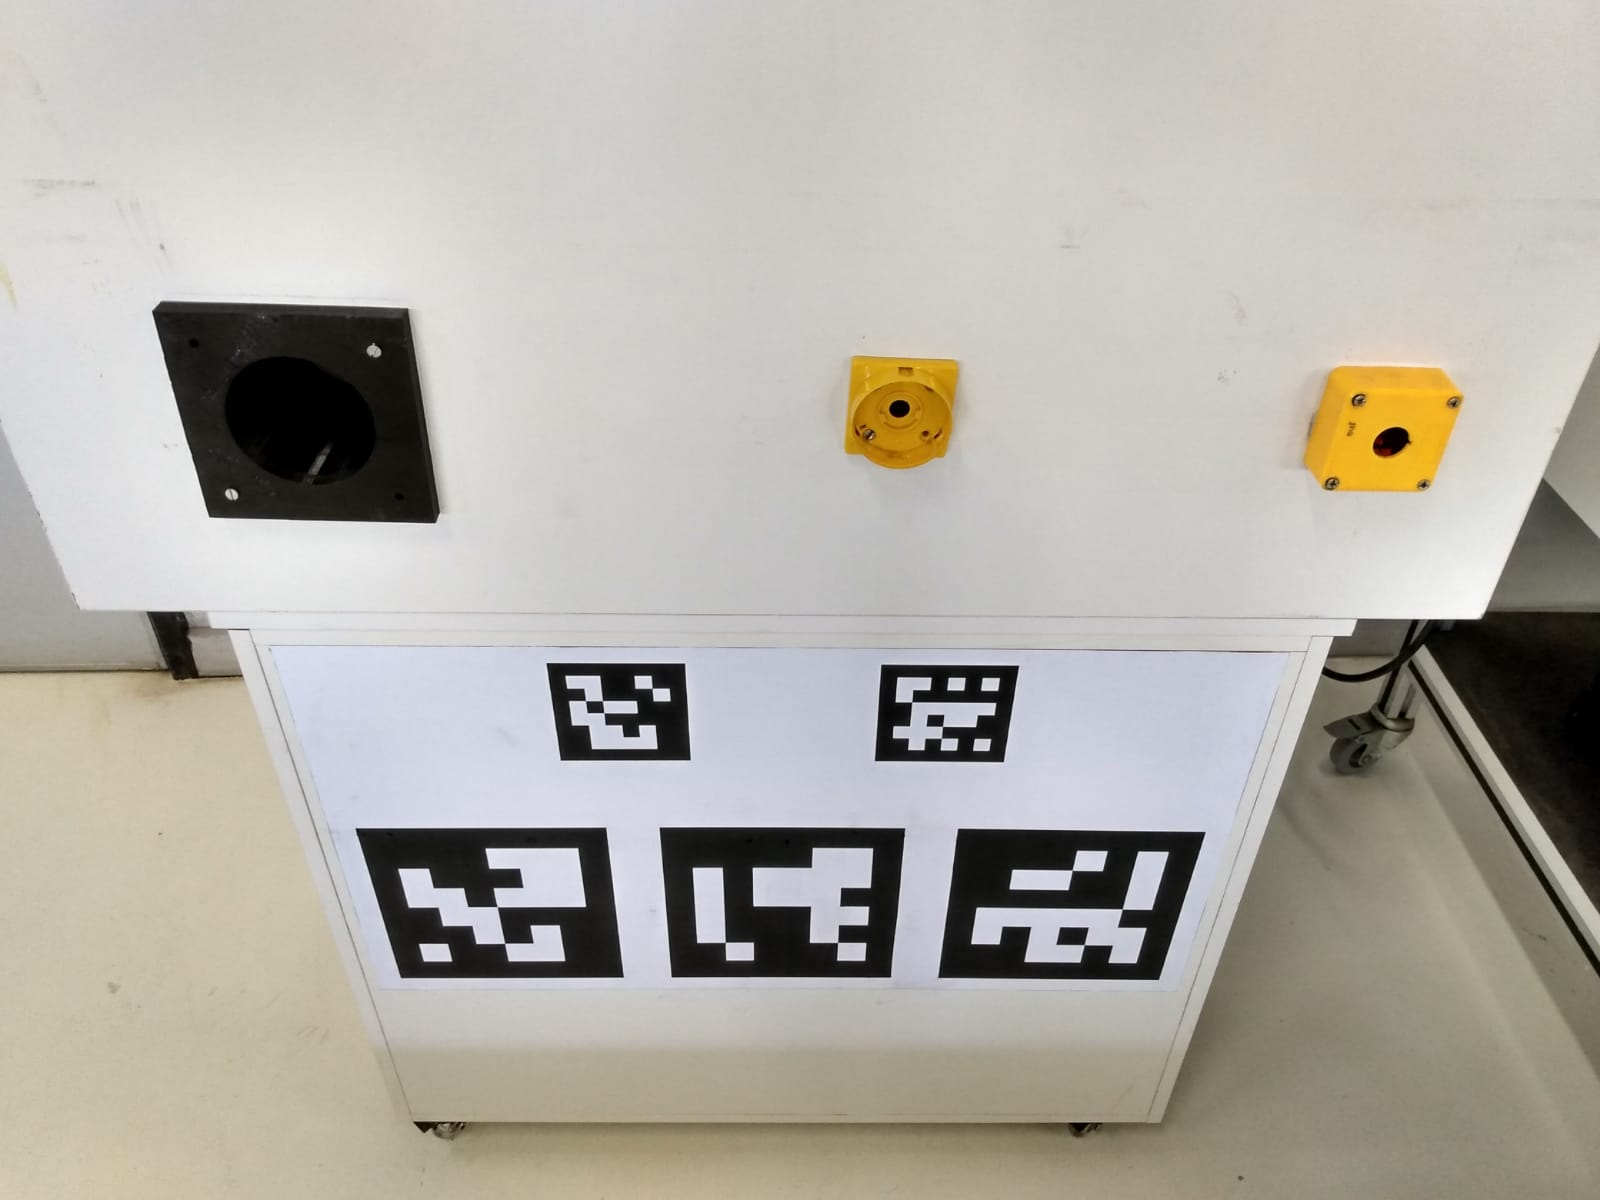
\includegraphics[width=.9\textwidth]{warthog+aum/aruco.jpeg}
            \end{figure}
        \end{center}

    \end{columns}

\end{frame}
%-

%*----------- SLIDE -------------------------------------------------------------
\begin{frame}[t]{Modelo para planejar trajetórias dinâmicamente} 
   
    \begin{columns}[c]
        \column{.6\textwidth}

            Etapas do modelo:
            \begin{itemize}
                \item \textbf{missão}: tarefa a ser executada pelo manipulador
                \item \textbf{abortar}: cancela a operação
                \item \textbf{solucionador}: soluciona a cinemática do robô
                \item \textbf{planejador}:  planeja a trajetória do robô 
                \item \textbf{preditor}: prever as posições futuras do  end-effector
            \end{itemize}
        \column{.4\textwidth}
            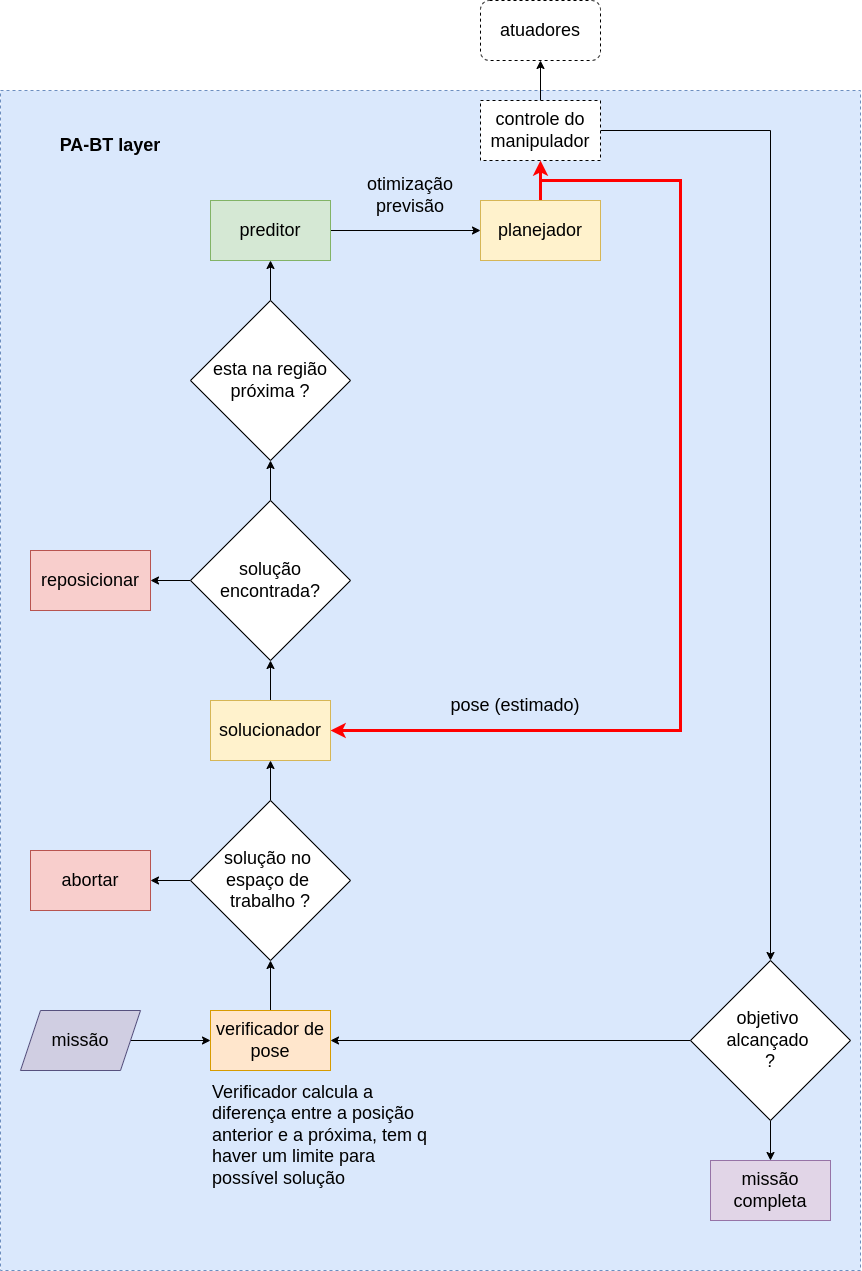
\includegraphics[width=0.8\textwidth]{warthog+aum/modelo-planejamento-dinamico.png}
    \end{columns}

\end{frame}
%-
%*----------- SLIDE -------------------------------------------------------------
\begin{frame}[t]{Teste UR5 com o MoveIt!} 
    \vspace*{0.3cm}
    \centering
    \begin{columns}[c]
        \column{.5\textwidth}
 
        O \textbf{MoveIt!} é um pacote do \textbf{ROS} voltado para as funcionalidades dos \textbf{manipuladores}. 

        \vspace*{0.3cm}
        Algumas funcionalidades do pacote
        \begin{itemize}
            \item Realizar o cálculo da cinemática
            \item Fazer o planejamento de trajetórias
            \item Verificar a presença de obstáculos
        \end{itemize}
        \vspace*{0.3cm}

        \column{.5\textwidth}
        \centering
        
\includegraphics[width=0.4\textwidth]{warthog+aum/moveit.png}

        \vspace*{0.8cm}

        \includemedia[
          width=1\linewidth,
          totalheight=0.39375\linewidth,
          activate=pageopen,
          passcontext, 
          addresource=./Source/movies/aum.mp4,
          flashvars={
          source=./Source/movies/aum.mp4
          &autoPlay=true
          &Loop=true}
          ]{\fbox{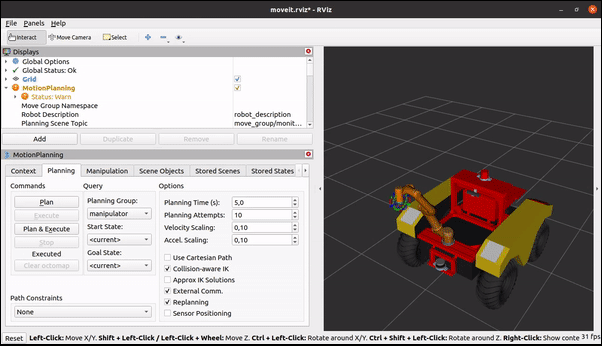
\includegraphics{warthog+aum/capa-aum.png}}}{VPlayer.swf}
    
    \end{columns}
    % \centering
    % 
\includegraphics[width=0.4\textwidth]{warthog+aum/moveit.png}

\end{frame}
%-
%*----------- SLIDE -------------------------------------------------------------
\begin{frame}[t]{Testes com o manipulador} 

    \begin{itemize}
        \item Reconhecimento dos arucos
        \item Deslocamento para as posições determinadas
        \item Coleta de dados para validação do script do preditor
    \end{itemize}
    \vspace*{0.6cm}
    \begin{columns}[c]
        \column{.5\textwidth}

        \centering

        \includemedia[
            width=0.7\linewidth,
            totalheight=0.39375\linewidth,
            activate=pageopen,
            passcontext, 
            addresource=./Source/movies/aum-aruco.mp4,
            flashvars={
            source=./Source/movies/aum-aruco.mp4
            &autoPlay=true
            &Loop=true}
            ]{\fbox{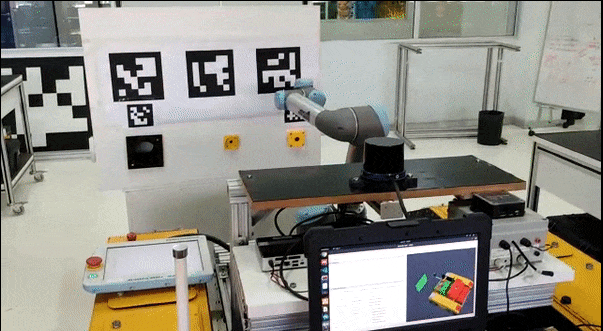
\includegraphics{warthog+aum/capa2.png}}}{VPlayer.swf}


        \column{.5\textwidth}
        \centering

        \includemedia[
          width=0.7\linewidth,
          totalheight=0.39375\linewidth,
          activate=pageopen,
          passcontext, 
          addresource=./Source/movies/aum-aruco1.mp4,
          flashvars={
          source=./Source/movies/aum-aruco1.mp4
          &autoPlay=true
          &Loop=true}
          ]{\fbox{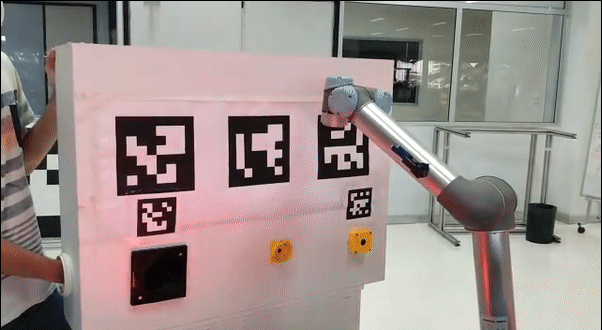
\includegraphics{warthog+aum/capa1.png}}}{VPlayer.swf}
    \end{columns}

\end{frame}
%-
%*----------- SLIDE -------------------------------------------------------------
\begin{frame}[t]{Modelo para planejar trajetórias dinâmicamente} 
    \vspace*{0.5cm} 
    \begin{columns}[c]
        \column{.5\textwidth}
        Ao reconhecer o \textbf{aruco} são obtidas as informações da sua \textbf{pose} (posição e orientação).

        \vspace*{0.3cm} 
        
        Nos testes realizados o manipulador tem como referência de objetivo para posicionar o seu \textbf{end-effector} a posição do aruco.
        \column{.5\textwidth}
        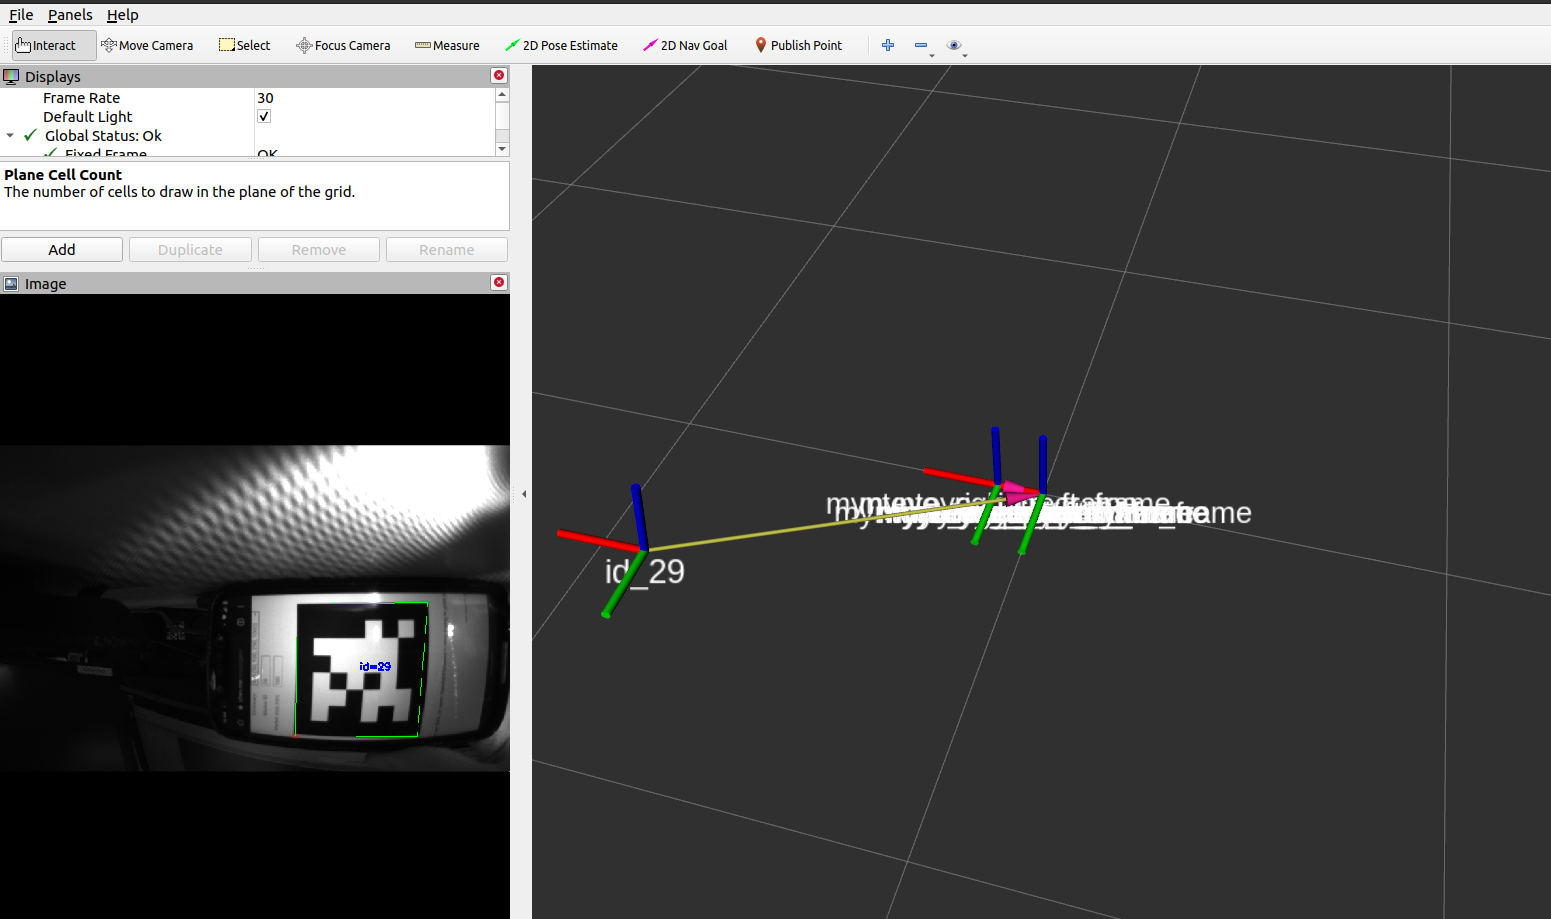
\includegraphics[width=.9\textwidth]{warthog+aum/Captura_de_tela_de_2021-10-15_16-44-28.png}
    \end{columns}

\end{frame}
%-
%*----------- SLIDE -------------------------------------------------------------
\begin{frame}[t]{Resultados obtidos do script do preditor} 

    \begin{columns}[t]
        \column{.01\linewidth}
        \column{.3\linewidth}
        \begin{center}
            Posições do eixo \textit{x} do aruco
            \begin{figure}
            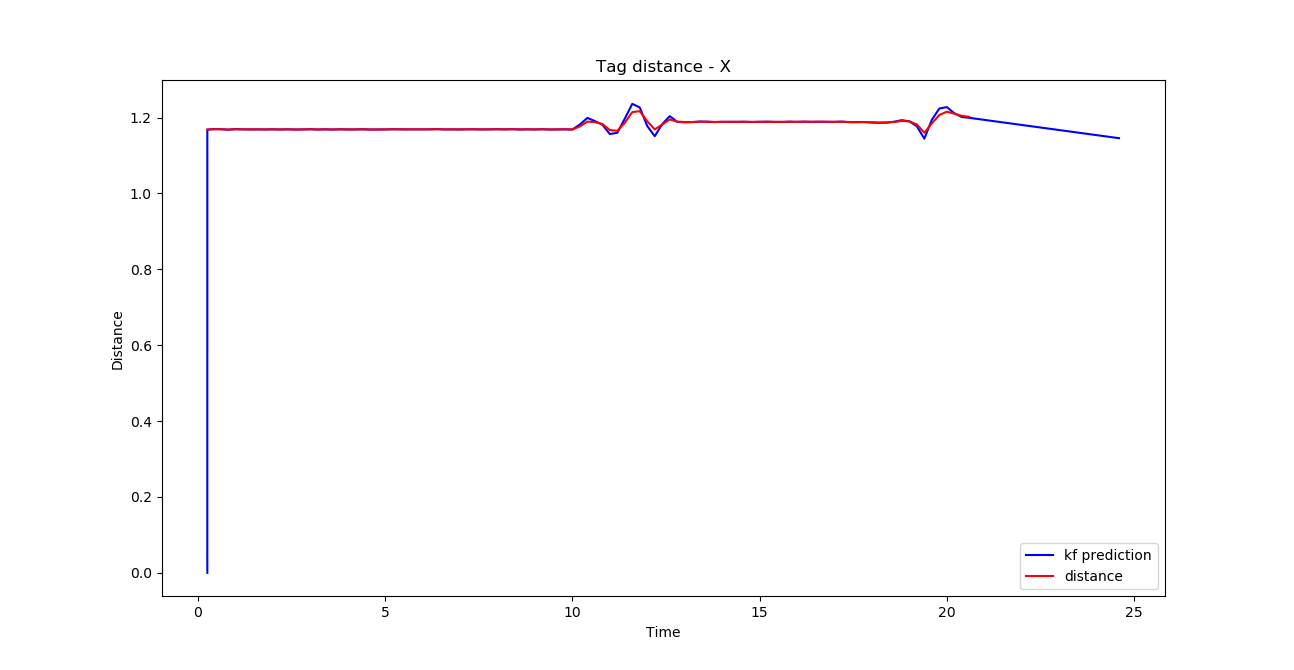
\includegraphics[width=.992\textwidth]{warthog+aum/x.png}
        \end{figure}
        \end{center}

        \column{.3\linewidth}
        \begin{center}
            Posições do eixo \textit{y} do aruco
            \begin{figure}
                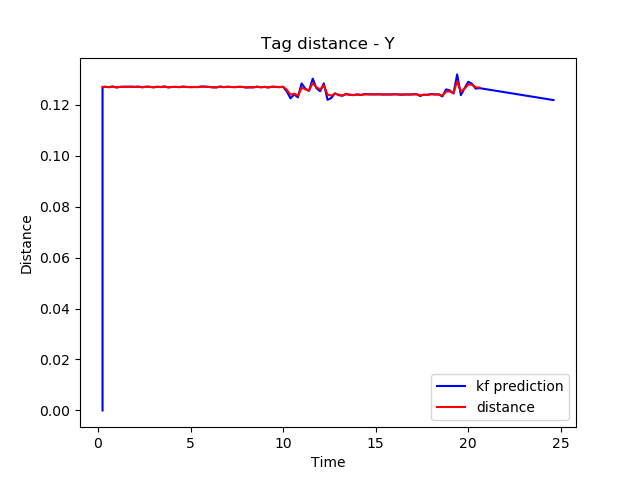
\includegraphics[width=.9\textwidth]{warthog+aum/y.png}
            \end{figure}
        \end{center}

        \column{.3\linewidth}
        \begin{center}
            Posições do eixo \textit{z} do aruco
            \begin{figure}
                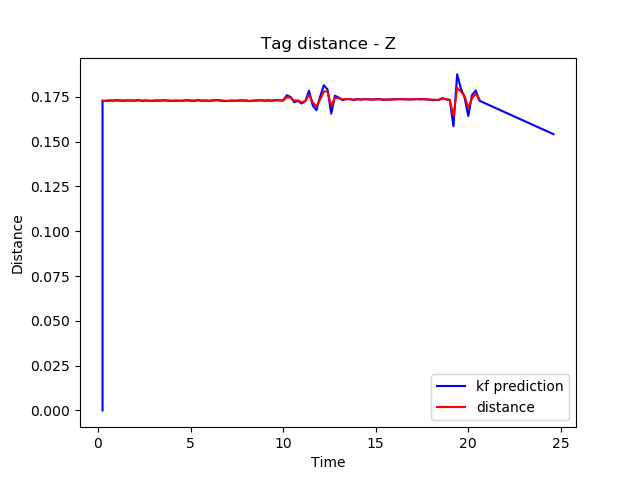
\includegraphics[width=.9\textwidth]{warthog+aum/z.png}
            \end{figure}
        \end{center}

    \end{columns}

\end{frame}
%-
%*----------- SLIDE -------------------------------------------------------------
\begin{frame}[t]{Considerações finais} 

    
    \vspace*{0.3cm}
    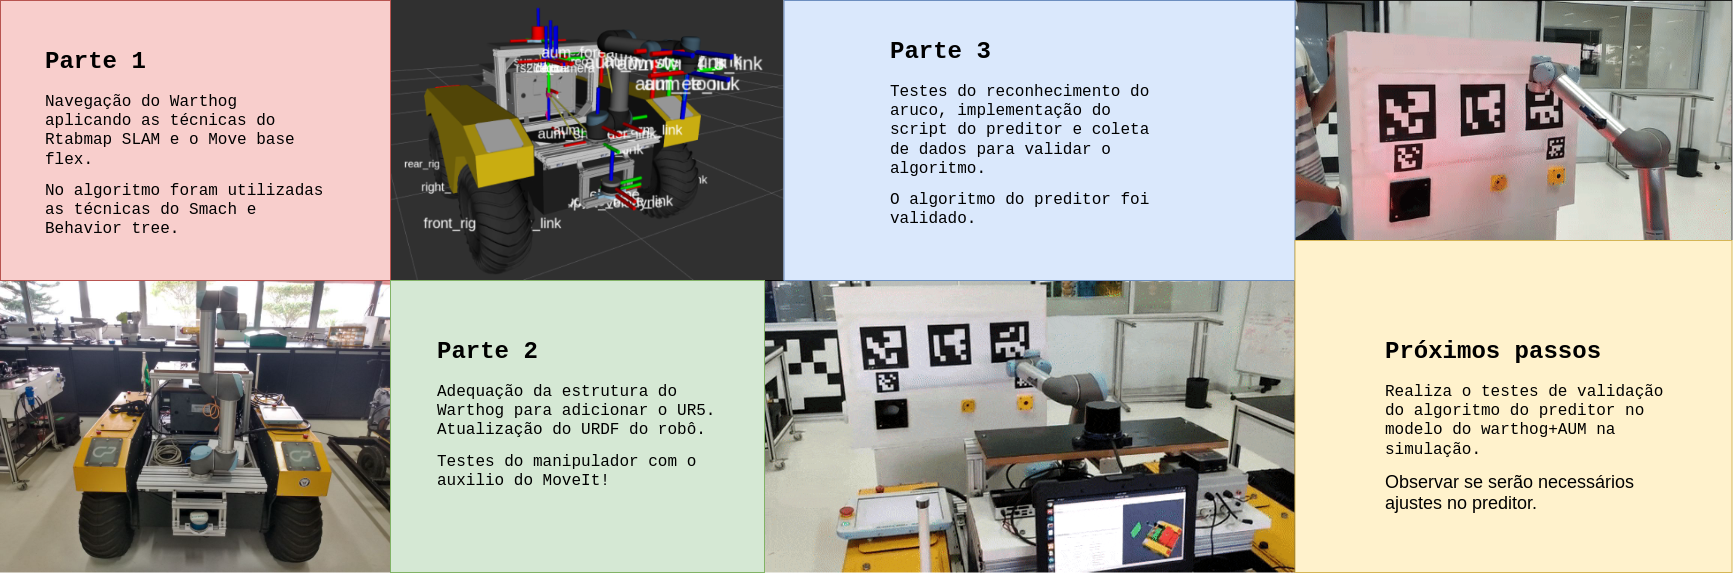
\includegraphics[width=1\textwidth]{warthog+aum/img-final.png}
%*----------- notes
    \note[item]{Notes can help you to remember important information. Turn on the notes option.}
\end{frame}
%-